%------------------------------------------------------------------------------
% Beginning of journal.tex
%------------------------------------------------------------------------------
%
% AMS-LaTeX version 2 sample file for journals, based on amsart.cls.
%
%        ***     DO NOT USE THIS FILE AS A STARTER.      ***
%        ***  USE THE JOURNAL-SPECIFIC *.TEMPLATE FILE.  ***
%
% Replace amsart by the documentclass for the target journal, e.g., tran-l.
%
\documentclass{amsart}

%     If your article includes graphics, uncomment this command.
\usepackage{graphicx}
% move author affiliations around
\usepackage{amsaddr}
\usepackage{amsfonts}
\usepackage{amsmath}% 
\usepackage{calc}%     needed for the width/height calculations
%resume enumerations
\usepackage{enumitem}


\newtheorem{theorem}{Theorem}[section]
\newtheorem{lemma}[theorem]{Lemma}

\theoremstyle{definition}
\newtheorem{definition}[theorem]{Definition}
\newtheorem{example}[theorem]{Example}
\newtheorem{xca}[theorem]{Exercise}

\theoremstyle{remark}
\newtheorem{remark}[theorem]{Remark}

\numberwithin{equation}{section}

%    Absolute value notation
\newcommand{\abs}[1]{\lvert#1\rvert}

%    Blank box placeholder for figures (to avoid requiring any
%    particular graphics capabilities for printing this document).
\newcommand{\blankbox}[2]{%
  \parbox{\columnwidth}{\centering
%    Set fboxsep to 0 so that the actual size of the box will match the
%    given measurements more closely.
    \setlength{\fboxsep}{0pt}%
    \fbox{\raisebox{0pt}[#2]{\hspace{#1}}}%
  }%
}

% Variable definitions
\def\T{$\mathcal{T}$}
\def\C{$\mathcal{C}$}
\def\TtoB{$\mathcal{T}2\mathcal{B}$}
\def\TSolver{$\mathcal{T}$-\emph{solver}}
\def\sat{\texttt{SAT}}
\def\unsat{\texttt{UNSAT}}
% \newcommand{\eqdef}{\overset{\mathrm{def}}{=\joinrel=}}


% \newcommand*{\MyDef}{\mathrm{def}}
% \newcommand*{\eqdefU}{\ensuremath{\mathop{\overset{\MyDef}{=}}}}% Unscaled version
% \newcommand*{\eqdef}{\mathop{\overset{\MyDef}{\resizebox{\widthof{\eqdefU}}{\heightof{=}}{=}}}}

\newcommand\eqdef{\mathrel{\overset{\makebox[0pt]{\mbox{\normalfont\tiny\sffamily def}}}{=}}}


\begin{document}

  \title[Satisfiability Modulo the Theory of Costs]{Satisfiability Modulo the Theory of Costs: Foundations and Applications}

  %    Information for first author
  \author{Marty Pye}
  \address{RWTH Aachen University}
  \email[Marty Pye]{marty.pye@rwth-aachen.de}

  \begin{abstract}
    This paper presents an overview of the modelling and evaluation of a theory of costs \C{} which extends Satisfiability Modulo Theories (SMT). This theory of costs allows modelling of domains which involve multiple cost functions and reasoning about resource consumption. This paper presents a decision procedure for the theory of costs by Cimatti et al.\ and explains the involved algorithm through the aid of a concrete example. How the theory of costs can help in tackling problems of optimisation modulo theories is also explained.
    \\\\
    An evaluation of the proposed approach in comparison to other solvers in the respective field is presented, and the results are discussed. They show that the presented decision procedure for cost problems is a competitive solution, and even outperforms existing solvers in certain cases.
  \end{abstract}

  \maketitle

  \section{Introduction}

  Very often, problems require modeling and constraining of resource consumption. This paper elaborates on an extension of SMT, a theory of costs, introduced by Cimatti et al.\ \cite{Cimatti10}. Problems modelled with the theory of costs can contain multiple cost functions, which can have upper and lower bounds, and depend on other boolean functions. The decision procedure they present has all the features required for the integration into the lazy SMT schema. This is based on the combination of a \sat{} solver and a theory solver, where the \sat{} solver handles the Boolean components and the theory solver handles the theory-specific components. The \sat{} solver enumerates truth assignments which satisfy the boolean abstraction of the input formula, while the theory solver checks the consistency within the theory \cite{Sebastiani07}. \\
  
  Based on the theory of costs, the problem of Optimisation Modulo Theories can be handled, either by a linear approach or by a binary search approach. The linear approach tightens the admissibility range based on the best valued solution so far, whereas the binary search approach bisects the admissible interval.
  Implementations of the proposed approaches are evaluated in comparison to other existing solvers, and the results are discussed. They show that both approaches are pretty effective.\\
  
  This thesis is structured as follows: In section \ref{smtSolving}, SMT solving is briefly explained, and in section \ref{theoryOfCosts} and \ref{theoryOfCosts2}, the theory of costs is introduced. A decision procedure for the theory of costs is presented and explained by use of a concrete example in section \ref{CSolver}. Finally, the solver is evaluated in section \ref{evaluation} with regards to existing solvers.

  \section{SMT Solving}
    \label{smtSolving}
    \emph{Satisfiability Modulo Theories} (SMT($\mathcal{T}$)) is a decision problem for first-order logic formulas with respect to some decidable first-order theory $\mathcal{T}$, and can be seen as a constraint satisfaction problem.
    A tool able to decide this problem is referred to as a SMT($\mathcal{T}$)-solver. A theory solver for a theory $\mathcal{T}$ can decide the satisfiability in $\mathcal{T}$ of sets and conjunctions of formulas, and is referred to as a $\mathcal{T}$-\emph{solver}.
    If the input set of \T{}-literals $\mu$ is satisfiable under \T{}, then the \TSolver{} returns \sat{}.
    Additionally, the \TSolver{} can return a so-called \T{}-deduction clause. This can be used in early pruning, where the \T{}-deduction clause can be used in backjumping and learning.
    If the input set of \T{}-literals is not satisfiable under \T{}, then the \TSolver{} returns \unsat{} and the conflict clause consisting of the subset of \T{}-literals in $\mu$ which was found \T{}-unsatisfiable.
    \\\\
    Let $\varphi$ denote a \T{}-formula, and \TtoB{}$(\varphi)$ its boolean abstraction. In a lazy SMT(\T{})-solver, the truth assignments for \TtoB{}$(\varphi)$ are checked for \T{}-satisfiability.
    Usually, this is performed by modified versions of the DPLL algorithm \cite{Davis60}. The basic DPLL algorithm runs by choosing a literal and assigning a truth value to it. It then simplifies the formula and  recursively checks whether the simplified formula is satisfiable.
    If this is the case, the original formula is satisfiable. Otherwise, the same recursive check is performed assuming the opposite truth value.
    If a truth assignment $\mu$ is found where \TtoB{}$(\mu) \models$ \TtoB{}$(\varphi)$ holds, then the respective constraints are passed on to the \TSolver{}.
    If the \TSolver{} then returns \sat{}, the SMT(\T{})-solver found a solution.
    If not, then the \TSolver{} passes the \T{}-conflict clause $\neg\eta$ back to the learning mechanism of the DPLL algorithm. For more information on how lazy SMT(\T{}) solving works, please refer to \cite{Sebastiani07}.

  \section{Satisfiability Modulo the Theory of Costs}
  \label{theoryOfCosts}
    Cimatti et al.\ extend the SMT framework by adding a possibility of modelling cost functions \cite{Cimatti10}.
    One cost function basically corresponds to the accumulative costs for a specific variable (e.g.\ battery, time, etc.). The cost function is built up of constraints, and (not) satisfying these leads to an increase (decrease) of the sum value of that cost function. Cost functions allow for things like ``flashing a torch causes $0.1\%$ of battery to be consumed'' to be modelled. They can be formally defined as follows:
    \\\\ 
    An SMT(\T{}) \emph{cost problem} is a pair $\langle \varphi, costs \rangle$, where $costs \eqdef \{cost^{i}\}^{M}_{i=1}$.
    In this pair, $\varphi$ is a boolean formula over ground \T{}-atoms and atoms of the form ($cost^{i} \leq c$), $c$ being some integer value. In the array $costs$, each $cost^{i}$ is a boolean cost function in the form
    \begin{equation}
      \label{eq:costsGeneral}
    	cost^{i} = \sum\limits_{j=1}^{N_{i}} (\text{if }\psi^{i}_{j} \text{ then }c^{i}_{j1} \text{ else }c^{i}_{j2})
    \end{equation}
    % where $ite$ (if-then-else) is a function defined as
    % \[
    %   ite(A,c_{1},c_{2}) = 
    % 	\begin{cases}
    %     c_{1},& \text{if } A = 1 \\
    %     c_{2},& \text{otherwise}
    % 	\end{cases}
    % \]
    where $\psi_{j}^{i}$ is a formula in \T{}. From here onwards, problems $\langle \varphi, costs \rangle$ are restricted s.t.
    \begin{equation}
    \label{eq:costsRestricted}
    	cost^{i} = \sum\limits_{j=1}^{N_{i}} (\text{if }A^{i}_{j} \text{ then }c^{i}_{j} \text{ else }0)
    \end{equation}
    where $A_{j}^{i}$ is a boolean literal and $0 < c^{i}_{j} \leq c^{i}_{j+1}$.
    Passing from ~\eqref{eq:costsGeneral} to ~\eqref{eq:costsRestricted} is straightforward and possible in linear time.
    \\\\
    At this point it is important to note that ~\eqref{eq:costsRestricted} can be encoded in the theory of linear arithmetic over integers ($\mathcal{LA}(\mathbb{Z})$) and therefore any $\langle \varphi, costs \rangle$ problem into the following \T{}$\cup \mathcal{LA}(\mathbb{Z})$-formula.
    \begin{equation}
    	\label{eq:encodingSMTIntoLA}
    	\langle \varphi, costs \rangle \equiv \varphi \bigwedge\limits_{i=1}^{M}\left(\left(c^{i} = \sum\limits_{j=1}^{N_{i}}c_{ij}\right) \land \bigwedge\limits_{j=1}^{N_{i}}\left(\left(A^{i}_{j} \to c_{ij} = c^{i}_{j}\right) \land \left(\neg A^{i}_{j} \to c_{ij} = 0\right)\right)\right)
    \end{equation}
    where $\left(A^{i}_{j} \to c_{ij} = c^{i}_{j}\right)$ and $\left(\neg A^{i}_{j} \to c_{ij} = 0\right)$ basically create summands, which are included into the accumulated cost sum, just like in ~\eqref{eq:costsRestricted}.
    The formula could then be solved by a linear arithmetic solver, such as \cite{dutertre06}. In practice however, this technique is extremely inefficient.
    In order to check whether $c^i$ is within a certain lower and upper bound, all the boolean literals $A^i_j$ need to be assigned, even when after adding a few $c^i_j$ it becomes clear that violating the upper bound cannot be avoided.
    The following theory of costs is more efficient to solve.

  \section{A Theory of Costs}
  \label{theoryOfCosts2}
    Cimatti et al.\ introduced a theory of costs $\mathcal{C}$, which allows for modelling multiple problems with $\mathcal{T} \cup \mathcal{C}$-formulas.
    \C{} is built up as follows:\\
    \begin{itemize}
      \item A set of $M$ variables $c^1,\ldots,c^M$. These are the output of the boolean cost functions $cost^1,\ldots,cost^M$.
      \item A binary predicate \sf BC \rm (``bound cost'') which allows modelling of upper and lower bounds for cost functions. \sf BC \rm is defined s.t.\ $\operatorname{\sf BC \rm}(c^i,c) \eqdef (c^i \leq c)$ with $c^i$ being a cost variable and $c$ being an integer value.
      \item A ternary predicate $\operatorname{\sf IC \rm}$ (``incur cost'') which allows modelling situations were a specific situation causes costs. \sf IC \rm is defined s.t. $\operatorname{\sf IC \rm}(c^i,j,c^{i}_{j}) \eqdef c^{i}_{j}$ is added to $c^i$ as $j^{th}$ element in the sum ~\eqref{eq:costsRestricted}.\\
    \end{itemize}
    This theory of costs allows for modelling domains which involve multiple costs $c^i$ and their constraints.
    At this point, we would like to introduce an example of an autonomous rover. In order not to overcomplicate the explanation, the given example does not contain an underlying theory.
    Imagine a rover that can move around a $4\times4$ field of squares (Fig.\ \ref{fig:roverField}).
    A move from one square to a neighbouring square costs $20$ mAh.\\\\
    Now, we want to model this behaviour in boolean logic, so first, we define some new boolean predicates:

    \begin{align*}
      \operatorname{\sf p \rm}(x,y,t) &\eqdef \text{at point in time $t$, rover is at }(x,y) \\
      \operatorname{\sf move \rm}(x,y,x',y',t) &\eqdef \text{at point in time $t$, rover moves from $(x,y)$ to $(x',y')$} \\
      \operatorname{\sf nextTo \rm}(x,y,x',y') &\eqdef (x,y) \text{ is a horizontal or vertical neighbour of $(x',y')$}
    \end{align*}
    \begin{figure}[!t]
      \centering
      \includegraphics[width = 0.8\textwidth]{images/roverField.pdf}
      \caption{Example of an autonomous rover, which can move left, right, up and down on this $4 \times 4$ field. A move from one square to a neighbouring square costs $20$ mAh of battery.}
      \label{fig:roverField}
    \end{figure}
    
    \noindent Second, we define some formulas which model the behaviour of the rover in a finite amount of time steps $n$:
    \begin{itemize}
      \item At every point in time, the rover is somewhere on the field:
      \begin{equation*}
        \varphi_{position} \eqdef \bigwedge\limits_{t \in \{0,\ldots,n\}} \left(\bigvee\limits_{x,y \in \{0,\ldots,3\}} \operatorname{\sf p \rm}\left(x,y,t\right)\right)
      \end{equation*}

      \item At any point in time, the rover can only be on one square:
      \begin{equation*}
        \varphi_{noSplitPos} \eqdef \bigwedge_{\substack{t \in \{0,\ldots,n\} \\ x,y \in \{0,\ldots,3\}}} \left(\operatorname{\sf p \rm}\left(x,y,t\right) \rightarrow \bigwedge_{\substack{x',y' \in \{0,\ldots,3\} \\ x' \neq x \wedge y' \neq y}} \neg \operatorname{\sf p \rm}\left(x',y',t\right)\right)
      \end{equation*}

      \item Between two points in time, the rover either moves or stays on its current square:
      \begin{equation*}
        \varphi_{move} \eqdef \bigwedge_{\substack{t \in \{0,\ldots,n-1\} \\ x,y,x',y' \in \{0,\ldots,3\} \\ x' \neq x \lor y' \neq y}} \left( \operatorname{\sf p \rm}\left(x,y,t\right) \land \operatorname{\sf p \rm}\left(x',y',t+1\right) \rightarrow \operatorname{\sf move \rm}\left(x,y,x',y',t\right)\right) 
      \end{equation*}

      \item The rover can only move to neighbouring field, i.e.\ neither jump nor move diagonally:
      \begin{equation*}
        \varphi_{validMove} \eqdef \bigwedge_{\substack{t \in \{0,\ldots,n-1\} \\ x,y,x',y' \in \{0,\ldots,3\}}} \left(\operatorname{\sf move \rm}\left(x,y,x',y',t\right) \rightarrow \operatorname{\sf nextTo \rm}\left(x,y,x',y'\right)\right)
      \end{equation*}

      \item Moving one square costs $20$ mAh of energy:
      \begin{equation*}
        \varphi_{batteryCost} \eqdef \bigwedge_{\substack{t \in \{0,\ldots,n-1\} \\ x,y,x',y' \in \{0,\ldots,3\}}} \left(\operatorname{\sf move \rm}\left(x,y,x',y',t\right) \rightarrow \operatorname{\sf IC \rm}\left(battery,t,20\right)\right)
      \end{equation*}
    \\
    \end{itemize}
    Using this example, we can model different constraints, which we want to impose. For example, can the rover move from $(0,0)$ to $(3,2)$ in 5 steps, while not using more than $100$ mAh of battery? This can be expressed with the following formula:
    \begin{equation*}
      \begin{split}
        \varphi_{ex1} \eqdef \varphi_{position} &\land \varphi_{noSplitPos} \land \varphi_{move} \land \varphi_{validMove} \land \varphi_{batteryCost} \\ 
        &\land \operatorname{\sf p \rm}(0,0,0) \land \operatorname{\sf p \rm}(3,2,5) \land \operatorname{\sf BC \rm}(battery, 100)
      \end{split}
    \end{equation*}
    
    It is fairly intuitive that the above formula is satisfiable, one possible solution being the path depicted in figure \ref{fig:roverField}. However, the problem could be extended to be more complex, e.g., with different battery costs for each square on a $1000 \times 1000$ field, which would make the problem a lot less easier for a human to solve. Therefore, Cimatti et al.\ introduced a general decision procedure for the theory of costs, a so-called \C{}-solver. The following chapter introduces the \C{}-solver, and explains the use of the individual steps with the aid of the rover example.

  \section{\C{}-solver: A theory of costs solver}
    \label{CSolver}
    A \C{}-solver receives a truth assignment $\mu \eqdef \mu_{\mathcal{B}} \cup \mu_{\mathcal{T}} \cup \mu_{\mathcal{C}}$, but only selects the \C{}-relevant part. $\mu_{\mathcal{B}}$ is a set of boolean literals, $\mu_{\mathcal{T}}$ a set of \T{}-literals and $\mu_{\mathcal{C}} \eqdef \bigcup_{i=1}^M \mu_{\mathcal{C}}^i$ is a set of \C{}-literals. $\mu_{\mathcal{C}}^i$ is a set of cost function constraints which are active under the current truth assignment. Formally, the set $\mu_{\mathcal{C}}^i$ can be defined s.t.\ for every $i$:
    \begin{equation*}
      \begin{split}
        \mu_{\mathcal{C}^i} \eqdef \{&\operatorname{\sf BC \rm}(c^i,\operatorname{\sf ub \rm}_{(k)}^{i})\ |\ k \in \{1,...,K_i\}\} \cup \{\neg \operatorname{\sf BC \rm}(c^i,\operatorname{\sf lb \rm}_{(m)}^{i} - 1)\ |\ m \in \{1,...,M_i\}\} \\
        \cup \ \{&\operatorname{\sf IC \rm}(c^i,j,c^i_j)\ |\ j \in J^{i+}\} \cup \{\neg \operatorname{\sf IC \rm}(c^i,j,c^i_j)\ |\ j \in J^{i-}\}
      \end{split}       
    \end{equation*}
    where $\operatorname{\sf ub \rm}_{(1)}^{i},\ldots,\operatorname{\sf ub \rm}_{(K^i)}^{i}$ and $\operatorname{\sf lb \rm}_{(1)}^{i},\ldots,\operatorname{\sf lb \rm}_{(K^i)}^{i}$ are positive integer upper and lower bounds respectively. $J^{i+}$ and $J^{i-}$ are sets of indices s.t.\ $J^{i+} \cap J^{i-} = \emptyset$ and $J^{i+} \cup J^{i-} \subseteq \{1,\ldots,N_i\}$. Additionally, in order to enhance the readability of the algorithm, let
    \begin{equation*}
      \begin{split}
        \text{largest lower bound} \approx \operatorname{\sf lb \rm}_{max}^i &\eqdef \operatorname{\sf max \rm}(\operatorname{\sf lb \rm}_{(1)}^i,\ldots,\operatorname{\sf lb \rm}_{(M_i)}^i) \\
        \text{smallest upper bound} \approx \operatorname{\sf ub \rm}_{min}^i &\eqdef \operatorname{\sf min \rm}(\operatorname{\sf ub \rm}_{(1)}^i,\ldots,\operatorname{\sf ub \rm}_{(K_i)}^i) \\
        \text{$i$-th cost of $\mu$} \approx \operatorname{\sf CostOf_i \rm}(\mu) &\eqdef \sum\limits_{j \in J^{i+}}c^i_j \\
        \text{largest possible $i$-th cost of $\mu$} \approx \operatorname{\sf MCostOf_i \rm}(\mu) &\eqdef \sum\limits_{j=1}^{N_i}c^i_j - \sum\limits_{j \in J^{i-}} c^i_j  
      \end{split}
    \end{equation*}
    So the \C{}-solver takes the \C{}-relevant part $\mu_{\mathcal{C}} \eqdef \bigcup_{i=1}^M \mu_{\mathcal{C}}^i$ and for every $i$, checks whether $\mu^{i}_{\mathcal{C}}$ is \C{}-satisfiable. This is performed by the following algorithm, which contains 6 steps. Each step is introduced and then explained in relation to the autonomous rover example.
    \\
    \begin{enumerate}
      \item If $\operatorname{\sf lb \rm}_{max}^i > \operatorname{\sf ub \rm}_{min}^i$ then return \unsat{} and the \C{}-conflict clause
      \begin{equation*}
        \operatorname{\sf BC \rm}(c^i, \operatorname{\sf lb \rm}_{max}^i - 1) \vee \neg \operatorname{\sf BC \rm}(c^i, \operatorname{\sf ub \rm}_{min}^i)
      \end{equation*} \\
      Step (1) is pretty straight forward. If the highest lower bound is larger than the lowest upper bound for a certain cost, then obviously, the formula is not satisfiable. In the rover example, this would be the case for e.g.\ $\varphi_{ex1} \land \neg \operatorname{\sf BC \rm}(battery,110)$. The rover cannot simultaneously use at least $110$ mAh and at most $100$ mAh of battery. This is precisely what the conflict clause then expresses. \\

      \item If $\operatorname{\sf CostOf_i \rm}(\mu_{\mathcal{C}}^i) > \operatorname{\sf ub \rm}_{min}^i$ then return \unsat{} and the \C{}-conflict clause
      \begin{equation*}
        \neg \operatorname{\sf BC \rm}(c^i, \operatorname{\sf ub \rm}_{min}^i) \vee \bigvee\limits_{j \in K^{i+}} \neg \operatorname{\sf IC \rm}(c^i, j, c^i_j)
      \end{equation*}
      $K^{i+}$ being a minimal subset of $J^{i+}$ s.t.\ $\sum\limits_{j \in K^{i+}} c^i_j > \operatorname{\sf ub \rm}_{min}^i$. \\\\
      Step (2) describes that for the current truth assignment, the accumulated cost for one cost variable may not exceed the lowest upper bound. In $\varphi_{ex1}$ for example, the solver checks wether all the currently incurred costs ($20$ mAh for each step) sum up to more than $100$. If yes, then the solver specifies that either the lowest upper bound cannot be $100$, or at one of the previous steps, the rover wasn't allowed to incur the costs it did. \\

      \item If $\operatorname{\sf MCostOf_i \rm}(\mu_{\mathcal{C}}^i) < \operatorname{\sf lb \rm}_{max}^i$ then return \unsat{} and the \C{}-conflict clause
      \begin{equation*}
        \operatorname{\sf BC \rm}(c^i, \operatorname{\sf lb \rm}_{max}^i - 1) \vee \bigvee\limits_{j \in K^{i-}} \operatorname{\sf IC \rm}(c^i, j, c^i_j)
      \end{equation*}
      $K^{i-}$ being a minimal subset of $J^{i-}$ s.t.\ $\sum\limits_{j \in K^{i-}} c^i_j < \operatorname{\sf lb \rm}_{max}^i$. \\\\
      Step (3) is analogous to step (2), just for the highest lower bound, i.e.\ the maximal accumulatable cost for the current assignment must exceed the highest lower bound, otherwise the formula is not satisfiable. \\

    \end{enumerate}
    If none of the conditions $(1)$, $(2)$ or $(3)$ are fulfilled, then the \C{}-solver returns \sat{} and $\operatorname{\sf CostOf_i \rm}(\mu_{\mathcal{C}}^i)$ for every i. Also, the \C{}-solver can perform theory propagation as follows:
    \begin{enumerate}[resume]
      \item Every unassigned literal $\operatorname{\sf BC \rm}(c^i, \operatorname{\sf ub \rm}_{(r)}^i)$ with $\operatorname{\sf ub \rm}_{(r)}^i \geq \operatorname{\sf ub \rm}_{min}^i$ and every unassigned literal $\neg \operatorname{\sf BC \rm}(c^i, \operatorname{\sf lb \rm}_{(s)}^i - 1)$ with $\operatorname{\sf ub \rm}_{(s)}^i) \leq \operatorname{\sf lb \rm}_{max}^i)$ can be \C{}-deduced, i.e.\ added to the truth assignment:
      \begin{equation*}
        \begin{split}
          \mu_{\mathcal{C}}^i &\cup \{\operatorname{\sf BC \rm}(c^i, \operatorname{\sf ub \rm}_{(r)}^i)\} \\
          \mu_{\mathcal{C}}^i &\cup \{\neg \operatorname{\sf BC \rm}(c^i, \operatorname{\sf lb \rm}_{(s)}^{i} - 1)\}
        \end{split}
      \end{equation*} \\
      Step (4) is relevant for early pruning.
      An important feature of this solver is that it can also take partial truth assignments.
      In order to show how this step can be useful, we have to complicate the example $\varphi_{ex1}$ a bit. Let's assume we have the formula 
      \begin{equation*}
        \varphi_{ex1} \land (\psi_1 \lor \operatorname{\sf BC \rm}(battery, 80) \lor \psi_2)
      \end{equation*}
      and the \sat{}-solver has already decided that $\psi_1$ and $\psi_2$ need to be false.
      Therefore $\operatorname{\sf BC \rm}(battery, 80)$ has to be true, and the solver can deduce that the unassigned literal $\operatorname{\sf BC \rm}(battery, 100)$ is automatically also true.
      That literal is then added to the truth assignment (\C{}-propagated).
      This makes the solving process more efficient. \\

      \item If $\operatorname{\sf CostOf_i \rm}(\mu) \leq \operatorname{\sf ub \rm}_{min}^i$ but $\left(\mu_{\mathcal{C}^i} \cup \{\operatorname{\sf IC \rm}(c^i, j, c^i_j)\}\right) > \operatorname{\sf ub \rm}_{min}^i$ for any $j \not\in (J^{i+} \cup J^{i-})$, then $\neg \operatorname{\sf IC \rm}(c^i, j, c^i_j)$ can be \C{}-deduced and added to the truth assignment: $\mu_{\mathcal{C}}^i \cup \{\operatorname{\sf IC \rm}(c^i, j, c^i_j)\}$. \\\\
      \begin{figure}[!t]
        \centering
        \includegraphics[width = 0.4\textwidth]{images/roverField2.pdf}
        \caption{One possible path the \sat{}-solver might chose. The algorithm can detect that the current path would incur too many costs, and conclude that a different path must be chosen.}
        \label{fig:roverField2}
     \end{figure}
      Step (5) and (6) basically do the same thing for upper and lower bounds respectively. Assuming the SAT solver has currently chosen an assignment which makes the rover move along the path depicted in figure \ref{fig:roverField2}. At this point in time, $\operatorname{\sf CostOf_i \rm}(\mu)$ is still $100$, but the cost incurred for the next step exceeds this bound. Therefore, the solver can deduce and propagate that this cost may not be incurred. The SAT-solver will then deduce that due to $\varphi_{batteryCost}$, the rover may not make that move, and has to find a different path. \\

      \item If $\operatorname{\sf MCostOf_i \rm}(\mu) \geq \operatorname{\sf lb \rm}_{max}^i)$ but $\left(\mu_{\mathcal{C}^i} \cup \{\neg \operatorname{\sf IC \rm}(c^i, j, c^i_j)\}\right) < \operatorname{\sf lb \rm}_{max}^i$ for any $j \not\in (J^{i+} \cup J^{i-})$, then $\operatorname{\sf IC \rm}(c^i, j, c^i_j)$ can be \C{}-deduced and added to the truth assignment: $\mu_{\mathcal{C}}^i \cup \{\neg \operatorname{\sf IC \rm}(c^i, j, c^i_j)\}$. \\\\
    \end{enumerate}

    \noindent If the problem also had an underlying theory, it could be solved by an SMT(\T{} $\cup$ \C{})-solver. A DPLL algorithm generates truth assignments and both the \C{}-solver and the \T{}-solver can be invoked on each of them. If both solvers return \sat{}, then the problem is satisfiable. If one of them returns \unsat{} and a conflict clause, then that conflict clause can be used by the SMT(\T{} $\cup$ \C{})-solver for backjumping and learning.

  \section{Optimisation Modulo Theories}
  \label{optimisationModuloTheories}
    An SMT(\T{} $\cup$ \C{})-solver can also solve \emph{cost decision} and \emph{cost minimisation} problems.

    A \textbf{cost decision problem} is a triple $\langle \varphi, costs, bounds \rangle$, where $\varphi$ and $costs$ are defined as in section \ref{theoryOfCosts}, and $bounds \eqdef \{\langle \operatorname{\sf lb \rm}^i, \operatorname{\sf ub \rm}^i\rangle\}^M_{i = 1}$ with $\operatorname{\sf ub \rm}^i$ and $\operatorname{\sf lb \rm}^i$ being integer values. The decision problem can be encoded into SMT(\T{} $\cup$ \C{}):
    \begin{equation*}
      \varphi_{\mathcal{C}} \eqdef \land \bigwedge\limits_{i = 1}^M \left( \operatorname{\sf BC \rm}\left(c^i, \operatorname{\sf ub \rm}^i \right) \land \neg \operatorname{\sf BC \rm}\left(c^i, \operatorname{\sf lb \rm}^i - 1\right) \land \bigwedge\limits_{j = 1}^M \left( A^i_j \leftrightarrow \operatorname{\sf IC \rm}\left( c^i, j, c^i_j \right)\right) \right)
    \end{equation*}
    \\
    A \textbf{cost minimization problem} is a triple $\langle \varphi, costs, bounds \rangle$ with $\varphi$, $costs$ and $bounds$ defined as above. The problem involves finding a solution where the value of $cost^i$ is minimal for a given $i$. Cimatti et al.\ describe two approaches to find the minimal cost, one based on linear search, and the other based on binary search. For a description of the algorithms, please refer to \cite{Cimatti10}.
    \\\\
    The following section evaluates Cimatti's solver for different problems in comparison to existing solvers which can solve the same type of problems.

  \section{Evaluation}
    \label{evaluation}
    \begin{table}
      \label{tab:performance}
      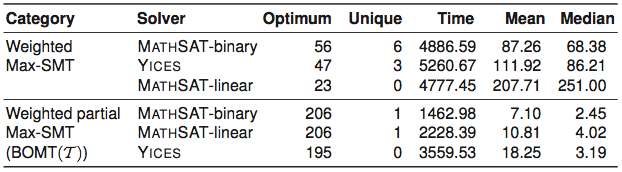
\includegraphics[width=0.8\linewidth]{images/performance.png}
      \caption{To be replaced with simpler table. The table shows the mean completion time of the different solvers and the number of instances where an optimal solution was found. The binary approach outperforms both the Yices SMT solver and the linear approach.}
    \end{table}

    Cimatti et al.\ evaluated the performance of their solver on problems which use a combination of \C{} and another theory \T{}. First, they evaluated their linear and binary approach in comparison to an SMT solver by Dutertre et al.\ \cite{yices06} on instances of the weighted Max-SMT and weighted partial Max-SMT problem. The \textbf{weighted Max-SMT} problem can be described as follows: For a given set of pairs $\{\left(C_1, c_1\right), \ldots, \left(C_m, c_m\right)\}$ where $C_i$ is an SMT clause weighted with cost $c_i$, find an assignment $\mu$ which maximises the sum $\sum_{i\ s.t.\ \mu \models C_i} c_i$ \cite{Nieuwenhuis06}. The \textbf{weighted partial Max-SMT} problem differentiates between hard and soft clauses. Only soft clauses are weighted with a cost. A solution is only valid iff it satisfies all hard clauses \cite{Robinson10}. Cimatti et al.\ ran the respective solvers on 200 instances of weighted (partial) Max-SMT problems, and compared the number of instances where optimal solutions were found as well as the completion time. The results showed that their binary approach outperformed the linear approach, finding 56 instances with optimal solutions as opposed to 23, and with a mean completion time of 87ms as opposed to 207ms. The exact results are listed in table 1.
    \\\\
    They also performed comparisons with Max-SAT solvers from the 2009 Max-SAT evaluation\footnote{http://www.maxsat.udl.cat/09/}. The results showed that for pure Max-SAT, neither their linear nor binary approach was competitive in finding optimal solutions. However, for weighted Max-SAT, the performance is noticeably better, and for weighted partial Max-SAT, their binary search approach is significantly better than the winner of the 2009 Max-SAT evaluation. The detailed results can be found in \cite{Cimatti10}. 

  \section{Conclusion}
    \label{conclusion}
    This paper provided an overview over a method of handling the problem of Satisfiability Modulo the Theory of Costs. The theory behind dealing with costs is introduced and explained with the help of a concrete example.
    The introduced SMT(\C{})-solver is an effective framework for solving optimisation problems.
    The solver and two approaches for optimisation problems, linear search and binary search, were evaluated. 
    Overall, the binary approach for the cost minimisation problem seems to find a larger number of optimal solutions than the linear approach.
    However, both the binary and linear approach find some solution for the same number of instances, as the first iteration of both algorithms is the same.
    The binary solver even outperforms the winners of the most recent competition in several categories. We can conclude that Cimatti's Satisfiability Modulo the Theory of Costs can handle expressive problems with multiple cost functions in an efficient way.



    
   
  \bibliographystyle{amsplain}
  \bibliography{references}

\end{document}

%------------------------------------------------------------------------------
% End of journal.tex
%------------------------------------------------------------------------------
